\usepackage[utf8]{inputenc}
\usepackage{slovak}
\usepackage{tikz}
\usetikzlibrary{arrows,positioning}
\usetheme{Warsaw}
\bibliographystyle{apalike}
\title{Decidability of Termination Problems for Sequential P Systems with Active Membranes}
\author{Michal Kováč}
\institute{FMFI UK, Slovakia}
\date{1.7.2015}
\begin{document}

\newcommand{\simulationpicture}{
  \tikzstyle{mybox} = [draw=black,very thick, rectangle, rounded corners, inner sep=10pt]
  \begin{tikzpicture}
    \onslide<2->{
      \node [mybox] (box){%
        \begin{minipage}{0.40\textwidth}
          \vspace{0pt}
          \begin{align}
            \tag{$r_1$}a\ |\ a &\rightarrow a\ |\ b\\
            \tag{$r_2$}a\ |\ b\ |\ b&\rightarrow b\\
            \tag{$r_3$}b &\rightarrow c
          \end{align}
          $a\ |\ a\ |\ b$
        \end{minipage}
      };
    }
    \onslide<3-4>{
      \node [mybox,below=3cm of box.west,anchor=west] (box2) {$a\ |\ b\ |\ c$};
      \path[-triangle 45] (box) edge [left] node {$r_1, r_3$} (box2);
    }
    \onslide<4-4>{
      \node [mybox,below=3cm of box.east,anchor=east] (box3){$a\ |\ c\ |\ c$};
      \path[-triangle 45] (box2) edge [above] node {$r_3$} (box3);
    }
    \onslide<6->{
      \node [mybox,below=3cm of box.east,anchor=east] (box2) {$a\ |\ b\ |\ b$};
      \path[-triangle 45] (box) edge [left] node {$r_1$} (box2);
    }
    \onslide<7->{
      \node [mybox,right=5cm of box.north,anchor=north] (box3){$a\ |\ a\ |\ c$};
      \path[-triangle 45] (box) edge [above] node {$r_3$} (box3);
    }
    \onslide<8->{
      \node [mybox,below=2cm of box3.west,anchor=west] (box4){$a\ |\ b\ |\ c$};
      \path[-triangle 45] (box2) edge [above] node {$r_3$} (box4);
      \path[-triangle 45] (box3) edge [left] node {$r_1$} (box4);
    }
    \onslide<9->{
      \node [mybox,below=2cm of box4.west,anchor=west] (box5){$a\ |\ c\ |\ c$};
      \path[-triangle 45] (box4) edge [left] node {$r_3$} (box5);
    }
    \onslide<10->{
      \node [mybox,below=3cm of box.west,anchor=west] (box6){$b$};
      \path[-triangle 45] (box2) edge [above] node {$r_2$} (box6);
    }
  \end{tikzpicture}
}

\begin{frame}[t]
\titlepage
\end{frame}
\note{}

\section*{Outline}
\begin{frame}
\tableofcontents
\end{frame}
\note{}

\section{P systems} % (fold)
\label{sec:p_systems}

  \subsection{Overview} % (fold)
  \label{sub:overview}

    \begin{frame}[t]\frametitle{Membrane structure}
      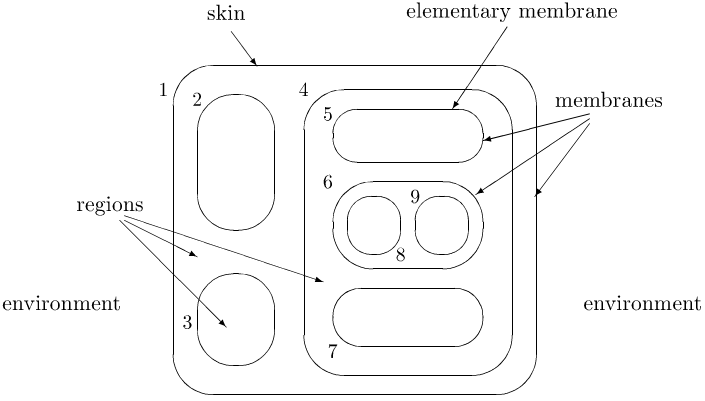
\includegraphics[width=0.7\textwidth]{membrane_structure.png}
      \hfill
      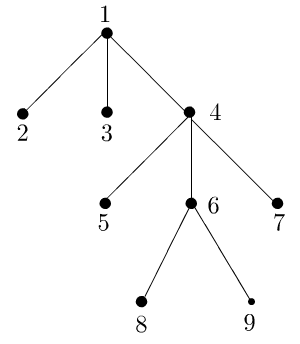
\includegraphics[width=0.3\textwidth]{membrane_tree.png}

    \end{frame}
    \note{}

    % \begin{frame}[t]\frametitle{Contents of the membrane}
    %   \begin{itemize}
    %     \item multiset of objects
    %     \begin{itemize}
    %       \item $a\ |\ b\ |\ b$
    %     \end{itemize}
    %     \item rewriting rules
    %     \begin{itemize}
    %       \item $a\ |\ b\ |\ b\rightarrow a\ |\ a_{out}\ |\ b_{in_{6}}$
    %       \item $b \rightarrow a\ |\ \delta$
    %     \end{itemize}
    %   \end{itemize}
    % \end{frame}
    % \note{}

    % \begin{frame}[t]\frametitle{P system}

    %   We define a P system as $\Pi = (V, \mu, w_1, w_2,\dots , w_m, R_1, R_2, \dots , R_m)$, where:
    %   \begin{itemize}
    %     \item $V$ is an alphabet of objects
    %     \item $\mu$ is a membrane structure
    %     \item $w_1, w_2, \dots w_m$ are initial multisets of objects in membranes $1\dots m$, $w_i\subseteq \mathbb{N}^V$
    %     \item $R_1, R_2, \dots , R_m$ are sets of rewriting rules in membranes $1\dots m$, where $$R_i\subseteq(\mathbb{N}^V\setminus 0^V)\times\mathbb{N}^{V\times(\{here,out\}\cup\{in_1,\dots in_m\})}$$.
    %   \end{itemize}

    % \end{frame}
    % \note{}

    \begin{frame}[t]\frametitle{Sequential vs. maximal parallel rule application}
      \begin{itemize}
        \item Sequential: in each step apply 1 rule
        \item Maximal parallel: in each step apply a maximal multiset of rules
      \end{itemize}
      \simulationpicture
    \end{frame}
    \note{}

    \begin{frame}[t]\frametitle{Language of a P system}
      \begin{itemize}
        \item The result of the computation is a multiset of objects, which is present in a specific membrane at a halting configuration
        \item The language generated by a P system is a set of results of all possible conputations.
      \end{itemize}
    \end{frame}
    \note{}
    \newpage
    \note{}

  % subsection overview (end)

  \subsection{Active membranes} % (fold)
  \label{sub:active_membranes}

    \begin{frame}[t]\frametitle{Variants of rules}
      \begin{itemize}
        \item cooperative ($a\ |\ b\ |\ b \rightarrow b$) (universal \cite{Paun98})
        \onslide<2->{\item non-cooperative ($b \rightarrow c$) (PsCF \cite{Sburlan05dragos})}
      \end{itemize}
    \end{frame}
    \note{}
    \newpage
    \note{}

    \begin{frame}[t]\frametitle{Sequential P systems}
      Sequential P systems with cooperative rules
      \onslide<2->{
        \begin{itemize}
          \item are equal to VASS $\Rightarrow$ not universal \cite{Dang:2005:Sequential}
          \item with priorities are universal \cite{Dang:2005:Sequential}
          \item with unbounded membrane creation are universal \cite{Dang:2005:Sequential}
          \onslide<3->{\item {\bf with inhibitors \cite{Kovac14}}}
        \end{itemize}
      }
    \end{frame}
    \note{}

  % subsection active_membranes (end)

% section p_systems (end)

\section{Termination problems} % (fold)
\label{sec:termination_problems}

  \subsection{Halting problem} % (fold)
  \label{sub:halting_problem}
  
    % \begin{frame}[t]\frametitle{Register machine}
    %   Minsky register machine is $M=(n,P,i,h)$, where:
    %   \begin{itemize}
    %     \item $n$ is the number of registers
    %     \item $P$ is a set of labeled instructions of type:
    %       \begin{itemize}
    %         \item $(add(r),k,l)$
    %         \item $(sub(r),k,l)$
    %         \item $halt$
    %       \end{itemize}
    %     \item $i$ is the initial instruction
    %     \item $h$ is the final instruction
    %   \end{itemize}
    % \end{frame}
    % \note{}

    \begin{frame}[t]\frametitle{Overview of the simulation for the accepting case}
      \begin{itemize}
        \item Simulation of a register machine
        \item Contents of register $j$ is represented by the multiplicity of the object $a_j$
        \item SUB instruction is simulated by inhibitors
      \end{itemize}
    \end{frame}
    \note{}

  % subsection halting_problem (end)

  \subsection{Termination problems in active membranes} % (fold)
  \label{sub:termination_problems_in_active_membranes}

    \begin{frame}[t]\frametitle{Overview of the simulation for the generating case}
      \begin{itemize}
        \item Simulation of a maximal parallel P system
        \item Start with the same rules
      \end{itemize}
      \simulationpicture
    \end{frame}
    \note{}

    \begin{frame}[t]\frametitle{Two phases}
      \begin{itemize}
        \item Prevent the rule application on already rewritten objects
          \onslide<2->{
            \begin{itemize}
              \item replace objects on the right side $a$ with $a^{\prime}$ 
              \item add $RESTORE$ phase
            \end{itemize}
            \onslide<3->{
              \item $RUN\ |\ a\ |\ a \rightarrow RUN\ |\ a^{\prime}\ |\ b^{\prime}$
              \item $RUN\ |\ a\ |\ b\ |\ b \rightarrow RUN\ |\ b^{\prime}$
              \item $RUN\ |\ b \rightarrow RUN\ |\ c^{\prime}$
            }
            \onslide<4->{
              \item $RESTORE\ |\ a^{\prime} \rightarrow RESTORE\ |\ a$
              \item $RESTORE\ |\ b^{\prime} \rightarrow RESTORE\ |\ b$
              \item $RESTORE\ |\ c^{\prime} \rightarrow RESTORE\ |\ c$
            }
          }
      \end{itemize}
    \end{frame}
    \note{}

    \begin{frame}[t]\frametitle{Switching the phases}
      \tikzstyle{mybox} = [draw=black,very thick, rectangle, rounded corners, inner sep=10pt]
      \begin{tikzpicture}
          \node [mybox] (box){RUN};
          \node [mybox,right=6cm of box.north,anchor=north] (box2){RESTORE};
          \path[-triangle 45] (box) edge [loop above] node {applying rules} (box);
          \path[-triangle 45] (box2) edge [loop above] node {restoring objects} (box2);
          \onslide<2->{
            \path[-triangle 45,bend left] (box) edge [above] node {no applicable rule} (box2);
            \path[-triangle 45,bend left] (box2) edge [below] node {all objects restored} (box);
          }
      \end{tikzpicture}
      \onslide<3->{
        \begin{itemize}
          \item $RUN\ |\ UNUSABLE_1\ |\ UNUSABLE_2\ |\ UNUSABLE_3 \rightarrow RESTORE$
          \onslide<4->{
            \item $RESTORE \rightarrow RUN\ |_{\neg{a^{\prime}b^{\prime}c^{\prime}}}$
          }
        \end{itemize}
      }
    \end{frame}
    \note{}

    \begin{frame}[t]\frametitle{Creating UNUSABLE objects (simple case)}
      \begin{itemize}
        \item $(3): b \rightarrow c$
        \item $RUN \rightarrow RUN\ |\ UNUSABLE_3\ |_{\neg{b,UNUSABLE_3}}$
      \end{itemize}
    \end{frame}
    \note{}

    \begin{frame}[t]\frametitle{Creating UNUSABLE objects (complicated case)}
      \begin{itemize}
        \item $(1): a\ |\ a \rightarrow a\ |\ b$
        \item $RUN \rightarrow RUN\ |\ UNUSABLE_1\ |_{\neg{a,UNUSABLE_1}}$
        \item Wrong for exactly 1 occurence of $a$
      \end{itemize}
    \end{frame}
    \note{}

    \begin{frame}[t]\frametitle{Promoting objects}
      \begin{itemize}
        \item $RUN\ |\ a \rightarrow RUN\ |\ \dot{a}\ |_{\neg{\dot{a}}}$
        \item $RUN\ |\ b \rightarrow RUN\ |\ \dot{b}\ |_{\neg{\dot{b}}}$
        \item $RUN\ |\ c \rightarrow RUN\ |\ \dot{c}\ |_{\neg{\dot{c}}}$
        \item At most 1 object can be promoted.
      \end{itemize}
    \end{frame}
    \note{}

    \begin{frame}[t]\frametitle{Using promoted objects}
      \begin{itemize}
        \item $RUN\ |\ a\ |\ \dot{a} \rightarrow a^{\prime}\ |\ b^{\prime}$
        \item $RUN\ |\ \dot{a}\ |\ b\ |\ b \rightarrow b^{\prime}$
        \item $RUN\ |\ \dot{a}\ |\ \dot{b}\ |\ b \rightarrow b^{\prime}$
        \item $RUN\ |\ a\ |\ \dot{b}\ |\ b \rightarrow b^{\prime}$
        \item $RUN\ |\ \dot{b} \rightarrow c^{\prime}$
        \onslide<2->{
          \item $RUN \rightarrow RUN\ |\ UNUSABLE_3\ |_{\neg{b,\dot{b},UNUSABLE_3}}$
          \item $RUN \rightarrow RUN\ |\ UNUSABLE_1\ |_{\neg{a, UNUSABLE_1}}$
        }
      \end{itemize}
    \end{frame}
    \note{}

    \begin{frame}[t]\frametitle{Multiple different objects on the left side}
      \begin{itemize}
        \item $(2): a\ |\ b\ |\ b \rightarrow b$
        \item $RUN \rightarrow RUN\ |\ UNUSABLE_2\ |_{\neg{a,\dot{a},UNUSABLE_2}}$
        \item $RUN \rightarrow RUN\ |\ UNUSABLE_2\ |_{\neg{b,UNUSABLE_2}}$
      \end{itemize}
    \end{frame}
    \note{}

    \begin{frame}[plain]
      \begin{center}
        Thanks for your attention!
      \end{center}
    \end{frame}

    \definecolor{run}{rgb}{1,0.5,0}
    \definecolor{restore}{rgb}{0,0.5,0}
    \definecolor{synchronize}{rgb}{0,0,1}
    \definecolor{senddown}{rgb}{1,0,0}
    % Narrow texts in boxes
    \providecommand{\narrow}[1]{\scalebox{.8}[1.0]{#1}}

  % subsection termination_problems_in_active_membranes (end)

% section termination_problems (end)


\newsavebox\mytempbib
\savebox\mytempbib{\parbox{\textwidth}{\bibliography{cie}}}

\end{document}
